\documentclass[conference]{IEEEtran}
\IEEEoverridecommandlockouts

% ---- packages ----
\usepackage{cite}
\usepackage{amsmath,amssymb,amsfonts}
\usepackage{amsthm}
\usepackage{algorithmic}
\usepackage{graphicx}
\usepackage{textcomp}
\usepackage{xcolor}
\usepackage{bm}
\usepackage{tikz}
\usetikzlibrary{arrows.meta,positioning,shapes.geometric,calc,decorations.pathmorphing,fit,backgrounds}
\usepackage[colorlinks=true,allcolors=blue]{hyperref}

\graphicspath{{figures/}}

% ---- theorem environments ----
\newtheorem{theorem}{Theorem}
\newtheorem{lemma}{Lemma}
\newtheorem{proposition}{Proposition}
\newtheorem{corollary}{Corollary}
\newtheorem{definition}{Definition}
\newtheorem{assumption}{Assumption}
\newtheorem{remark}{Remark}

% ---- notation macros ----
\newcommand{\R}{\mathbb{R}}
\newcommand{\Wten}{\mathcal{W}}          % (legacy alias; use \Wmap = support-capability map)
\newcommand{\Xwise}{\mathcal{X}_{\mathrm{WISE}}}
\newcommand{\lamtwo}{\lambda_2}
\newcommand{\Lap}{\bar L}                       % decision-induced candidate-site Laplacian
\newcommand{\Lgeo}{L_{\mathrm{geo}}}           % geometric (position-dependent) Laplacian
\newcommand{\Pot}{\Phi}
\newcommand{\wdem}{w^{\mathrm{dem}}}
\newcommand{\mF}{m_F}                     % strong-monotonicity constant
\newcommand{\PoE}{\mathrm{PoE}}
\newcommand{\Emanifold}{\mathcal{E}}          % optimal composition fiber (level set of the aggregate map)
\newcommand{\Ess}{\mathcal{E}_{\mathrm{ss}}}  % self-sustaining subset
\newcommand{\Lammax}{\Lambda^{\star}}         % max algebraic connectivity over E
\newcommand{\LamE}{\Lambda_{\Emanifold}}      % max lambda_2 over the optimal fiber E
\newcommand{\LamX}{\Lambda_{X}}               % max lambda_2 over the feasible set X_f
\newcommand{\Cdelta}{\mathcal{C}_{\delta}}    % safe information set {lambda_2 >= sigma_req}
\newcommand{\Ddelta}{\Delta_{\delta}}         % productive loss in the costly regime
\newcommand{\sigmadyn}{\sigma_{\mathrm{dyn}}} % dynamic stability threshold = theta^2/(c m_F)
\newcommand{\sigmastar}{\sigma_{\mathrm{req}}}% WISE-required threshold = sigma_dyn + delta
\newcommand{\vt}{\vartheta}                    % cross-coupling
\newcommand{\Wmap}{\mathcal{W}}                % directional support-capability map

\begin{document}

\title{WISE: Wrench- and Information-Self-Sustaining\\
Equilibrium Selection for Heterogeneous Multi-Robot Transport}

\author{\IEEEauthorblockN{Jorge Luis Mayorga Taborda}
\IEEEauthorblockA{\textit{Universidad Internacional de Valencia (VIU)}\\
Valencia, Spain\\
jl.mayorga236@gmail.com}}

\maketitle

\begin{abstract}
Distributed equilibrium-seeking controllers for multi-robot systems commonly assume
that the communication graph is available independently of the assignment being
computed. In cooperative transport, however, committing robots to lifting and relay
roles changes the graph itself. We formulate a relaxed heterogeneous
task-assignment model in which the wrench-feasible compositions that produce the same
optimal served aggregate form an \emph{equilibrium fiber}. A \emph{wrench- and
information-self-sustaining equilibrium} (WISE) is a point on this fiber whose
decision-induced candidate-site Laplacian $\Lap(z)$ meets a robust
algebraic-connectivity requirement. We characterize the fiber dimension on its
active face, cast WISE existence and selection as a semidefinite program, and derive
a sufficient spectral condition for exponential stability of the coupled
served-aggregate/estimator subsystem---also necessary in the isotropic modal case. A
lexicographic selector preserves the productive optimum exactly while maximizing
connectivity. Simulations with heterogeneous second-order unicycles evaluate the SDP
certificate, the predicted stability boundary, and a decentralized numerical
realization. The results separate wrench infeasibility from communication
infeasibility and show that relay allocation follows the spectral benefit of each
robot type relative to its productive opportunity cost.
\end{abstract}

\begin{IEEEkeywords}
Multi-robot systems, cooperative transport, task allocation, variational equilibria,
algebraic connectivity, semidefinite programming.
\end{IEEEkeywords}

\section{Introduction}
\label{sec:intro}

Cooperative transport by a heterogeneous robot team couples two decisions usually
studied apart: which robots apply force to a load, and which relay the information
that lets the team agree on that force. Distributed equilibrium-seeking and
population-game methods coordinate such teams by having each agent revise its
strategy from locally communicated aggregates, converging to an equilibrium of a
constrained potential game~\cite{sandholm2010population,quijano2017role,%
barreiro2016constrained,martinezpiazuelo2022}. These methods rest on one premise:
the communication graph needed to \emph{compute} the equilibrium is available while
the equilibrium is being reached.

For a mobile team this cannot be taken for granted: the robots that compute the
equilibrium are the robots whose placement forms the graph. An assignment can be productively
optimal---delivering the demanded wrench (force and torque~\cite{murray1994manipulation})---yet
commit every robot to lifting, leaving none to relay, so connectivity collapses and the
estimator loses its consensus channel.

Population-game and distributed Nash-seeking formulations take the interaction graph as
given~\cite{quijano2017role,barreiro2016constrained}. Communication-aware
task allocation couples the two, trading task utility against assignment-induced
connectivity~\cite{williams2017matroid,lin2021connectivity,zavlanos2011connectivity,%
ghosh2006growing}; recent heterogeneous MRTA solves integer coalition
allocation under physical constraints~\cite{calvo2025heterogeneous}, and communication-backbone
methods reconfigure the relay layer~\cite{santos2024backbone}. Each imposes connectivity as a
\emph{constraint}, scalarises it against task utility, or repairs the backbone after the fact.
To the best of our targeted review, none characterizes the geometry of the \emph{exact}
wrench-feasible productive-optimum set and uses its neutral directions to decide whether
connectivity is attainable at exactly zero productive loss.
We exploit a structural degeneracy: because
the payoff couples only through aggregates~\cite{jensen2010aggregative}, the productive
optimum fixes the served aggregate but leaves an aggregate-invariant fiber of
wrench-feasible compositions (Theorem~\ref{thm:degeneracy}), over which connectivity is
selected lexicographically.

\emph{What is and is not new.} The mechanics we invoke are standard---concavity of $\lamtwo$
in affine weights~\cite{fiedler1973,ghosh2006growing}, directional derivatives of a repeated
minimum eigenvalue~\cite{lewis1996spectral,overton1992large}, LMI connectivity design, and
first-order optimality of a concave function over a convex set. The contribution is the object
they are applied to: that the wrench-feasible productive-optimum set is a positive-dimensional
polytope whose tangent cone carries the entire zero-loss connectivity question, condensed into
one computable scalar $\Gamma_{\Emanifold}$. \emph{Scope:} equilibrium-set geometry and
centralized target selection, not distributed Nash seeking.

\paragraph*{Contributions}
\begin{itemize}
\item \textbf{Active-face and tangent-cone geometry} (Theorem~\ref{thm:degeneracy},
Thm.~\ref{thm:networkability}): the optimal served aggregate is unique, but the equal-payoff
assignments form a fiber whose dimension is the local loss of strong monotonicity on the
minimal active face; a tangent-cone criterion certifies when connectivity improves at
\emph{zero} productive cost, including a repeated Fiedler eigenvalue.
\item \textbf{WISE threshold and price of self-sustainability}
(Theorems~\ref{thm:existence},~\ref{thm:price}): relaxed WISE existence and selection are a
lexicographic semidefinite program, and the spectral capacities $\LamE\le\LamX$ separate
\emph{free}, \emph{costly}, and \emph{impossible} requirements through a convex price
$\Price(\sigma)$ whose subgradient prices connectivity in units of utility.
\item \textbf{Finite-team assessment} (Proposition~\ref{prop:integer}): a deterministic but
conservative joint-feasibility radius, an exact small-team oracle, and a directly
re-certified structured recovery that together quantify integer attainability, recovery loss,
and the conservatism of the worst-case bound.
\end{itemize}
The guarantees are for the affine
relaxation; a reduced information-layer model (Prop.~\ref{thm:stability}) supplies the
connectivity requirement, and distributed online realization remains future work.

% Concept figure removed for the six-page limit (was uncited); source preserved in
% sections/fig_concept.tex and restorable for the extended/repository version.
% \begin{figure*}[t]\centering
% \resizebox{0.62\textwidth}{!}{% The self-defeating equilibrium, two stacked rows for clarity.
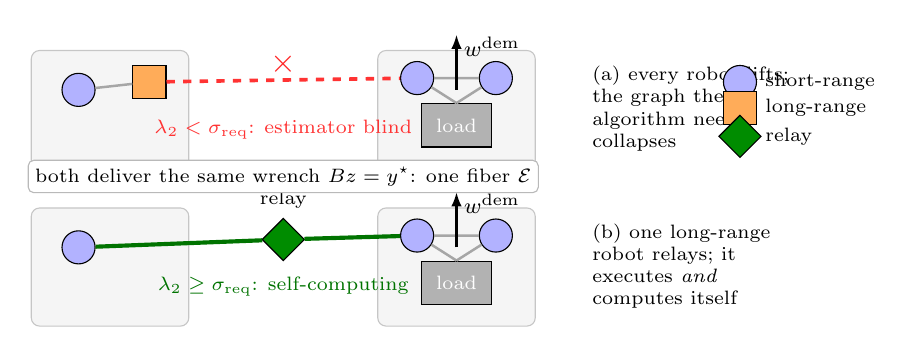
\begin{tikzpicture}[
  font=\footnotesize,
  short/.style={circle,draw=black,fill=blue!30,minimum size=4.2mm,inner sep=0pt},
  long/.style={rectangle,draw=black,fill=orange!65,minimum size=4.2mm,inner sep=0pt},
  rel/.style={diamond,draw=black,fill=green!55!black,minimum size=5.4mm,inner sep=0pt},
  ld/.style={rectangle,draw=black,fill=gray!60,text=white,font=\scriptsize,
             minimum width=9mm,minimum height=5.5mm,inner sep=0.5pt},
  cl/.style={rounded corners=3pt,draw=gray!45,fill=gray!8,inner sep=0pt},
  lk/.style={gray!70,line width=0.9pt},
  brk/.style={red!80,dashed,line width=1.3pt},
  brg/.style={green!45!black,line width=1.5pt},
  lab/.style={font=\scriptsize},
  x=1cm,y=1cm]

% ================= Row (a): self-defeating =================
\begin{scope}[yshift=2.0cm]
  \node[cl,minimum width=2.0cm,minimum height=1.5cm] at (1.0,0.7){};
  \node[cl,minimum width=2.0cm,minimum height=1.5cm] at (5.4,0.7){};
  % left cluster
  \node[short](a1) at (0.6,0.95){}; \node[long](a2) at (1.5,1.05){};
  \draw[lk] (a1)--(a2);
  % right cluster: load + lifters
  \node[ld](La) at (5.4,0.5){load};
  \node[short](a4) at (4.9,1.1){}; \node[short](a5) at (5.9,1.1){};
  \draw[lk] (a4)--(La.north) (a5)--(La.north) (a4)--(a5);
  \draw[-{Latex[length=1.8mm]},thick] (5.4,0.95)--(5.4,1.65);
  \node at (5.85,1.5){$\wdem$};
  % broken inter-cluster link
  \draw[brk] (a2)--(a4);
  \node[red!85] at (3.2,1.28){\large$\times$};
  \node[red!80,lab] at (3.2,0.45){$\lamtwo<\sigmastar$: estimator blind};
  \node[lab,anchor=west] at (7.0,0.7)
    {\begin{tabular}{@{}l@{}}(a) every robot lifts;\\ the graph the\\ algorithm needs\\ collapses\end{tabular}};
\end{scope}

% ================= Row (b): self-sustaining (WISE) =================
\begin{scope}
  \node[cl,minimum width=2.0cm,minimum height=1.5cm] at (1.0,0.7){};
  \node[cl,minimum width=2.0cm,minimum height=1.5cm] at (5.4,0.7){};
  \node[short](b1) at (0.6,0.95){};
  \node[ld](Lb) at (5.4,0.5){load};
  \node[short](b4) at (4.9,1.1){}; \node[short](b5) at (5.9,1.1){};
  \draw[lk] (b4)--(Lb.north) (b5)--(Lb.north) (b4)--(b5);
  \draw[-{Latex[length=1.8mm]},thick] (5.4,0.95)--(5.4,1.65);
  \node at (5.85,1.5){$\wdem$};
  % long-range robot diverted to relay in the gap
  \node[rel](br) at (3.2,1.05){}; \node[lab] at (3.2,1.55){relay};
  \draw[brg] (b1)--(br) (br)--(b4);
  \node[green!45!black,lab] at (3.2,0.45){$\lamtwo\ge\sigmastar$: self-computing};
  \node[lab,anchor=west] at (7.0,0.7)
    {\begin{tabular}{@{}l@{}}(b) one long-range\\ robot relays; it\\ executes \emph{and}\\ computes itself\end{tabular}};
\end{scope}

% ================= shared fiber note (between rows) + legend =========
\node[draw=gray!55,rounded corners=2pt,fill=white,inner sep=2.5pt,lab]
  at (3.2,1.85){both deliver the same wrench $Bz=y^{\star}$: one fiber $\Emanifold$};
% legend (top-right)
\node[short] at (9.0,3.05){}; \node[lab,anchor=west] at (9.2,3.05){short-range};
\node[long]  at (9.0,2.72){}; \node[lab,anchor=west] at (9.2,2.72){long-range};
\node[rel]   at (9.0,2.36){}; \node[lab,anchor=west] at (9.2,2.36){relay};
\end{tikzpicture}
}
% \caption{Assignment-induced connectivity and WISE selection: (1) the seeker computes $z$
% from aggregates over the graph $\Lap(z)$ that $z$ itself forms; (2) the productive optimum
% fixes $Bz=y^{\star}$ but not the composition, so a fiber $\Emanifold$ attains $V^{\star}$
% with $\lamtwo$ crossing $\sigmastar$; (3) a comparative-advantage long/short role exchange
% keeps $Bz=y^{\star},V^{\star}$ while moving $\lamtwo$ across $\sigmastar$.}
% \label{fig:scene}
% \end{figure*}
\section{Population Model and Induced Network}
\label{sec:model}

\subsection{Assignment state (relaxed robot counts $z$)}
A team of $N=\sum_\tau n_\tau$ robots is partitioned into $T$ types
$\tau\in\{1,\dots,T\}$ (heterogeneous in force capacity and communication range),
with $n_\tau$ robots of type $\tau$. There are $M$ loads with $H$ contact slots
each, a set $\mathcal R$ of candidate relay sites, and the common action set
\begin{equation}
\mathcal A=\underbrace{\{(k,h)\}_{k\le M,\,h\le H}}_{\text{load--slot}}
\;\cup\;\mathcal R\;\cup\;\{\mathrm{o}\},
\label{eq:actions}
\end{equation}
with $\mathrm o$ idle. We write $a\in\mathcal A$ for a generic action, $(k,h)$ for a
load--slot, and $r\in\mathcal R$ for a relay site.

The \emph{assignment state} is the relaxed-count matrix
$z=(z_{\tau a})\in\R_{\ge0}^{T\times|\mathcal A|}$: $z_{\tau a}$ is a continuous
relaxation of the number of type-$\tau$ robots assigned to action $a$---neither a
probability nor a physical force. Each type spends its budget, and each slot or
relay site holds at most one robot,
\begin{equation}
\begin{aligned}
&\textstyle\sum_{a\in\mathcal A} z_{\tau a}=n_\tau\ \ \forall\tau,
\qquad z_{\tau a}\ge0,\\[1mm]
&\textstyle\sum_\tau z_{\tau,kh}\le1\ \ \forall(k,h),
\qquad \sum_\tau z_{\tau,r}\le1\ \ \forall r.
\end{aligned}
\label{eq:conservation}
\end{equation}
The feasible set
$\mathcal X=\{z\in\R_{\ge0}^{T\times|\mathcal A|}:\eqref{eq:conservation}\}$ is a
compact convex polytope. A finite team instantiates $z$ by an integer assignment
(one action per robot); integerization is treated in Remark~\ref{rem:integer}. The
state $z$ is distinct from the physical poses $q\in(\mathrm{SE}(2))^N$, which enter
only the closed-loop simulation (Section~\ref{sec:exp}). Multiplying a count
$z_{\tau kh}$ by a per-robot force yields a total force, so every aggregate below is
dimensionally a force or torque.

\begin{assumption}[Standing hypotheses]\label{as:standing}
Throughout: \emph{(i)} $\mathcal X$ is compact and convex; \emph{(ii)} the aggregate
map $z\mapsto s(z)$ of \eqref{eq:tensor} is linear, so the wrench-feasible set
$\mathcal X_{\mathrm f}=\{z\in\mathcal X:s_{k\ell}(z)\ge d_{k\ell}\}$ is a polytope;
\emph{(iii)} the candidate-site Laplacian $\Lap(z)$ of \eqref{eq:laplacian} is affine
in $z$ with each elementary $L_e\succeq0$ and each coefficient $\ge0$; \emph{(iv)}
the communication graph is undirected and weighted, so every $\Lap(z)$ is a symmetric
graph Laplacian; and \emph{(v)} $\mathcal X_{\mathrm f}\neq\varnothing$.
\end{assumption}

\subsection{Support-function wrench certificate}
\emph{Physical force set.} A type-$\tau$ robot with heading $\phi$ exerts contact
forces in the heading-aligned ellipse $U_\tau(\phi)$ with longitudinal semi-axis
$F_\tau$ (along $\phi$) and lateral semi-axis $\kappa F_\tau$ ($\kappa\le1$, the
nonholonomic penalty). \emph{Certificate set.} The strategic layer does not track
headings, so for the certificate we use the heading-independent, centrally
symmetric \emph{inner} regular $2m$-gon $U_\tau^{\mathrm{in}}$ inscribed in the
disk of radius $\kappa F_\tau$. Since $\mathrm{disk}(\kappa F_\tau)\subseteq
U_\tau(\phi)$ for every $\phi$ (the ellipse's minimum semi-axis is $\kappa
F_\tau$), we have $U_\tau^{\mathrm{in}}\subseteq U_\tau(\phi)$ for all $\phi$;
feasibility tested against $U_\tau^{\mathrm{in}}$ is therefore \emph{conservative}
and cannot create a false positive.

Let $A_{kh}\in\R^{3\times2}$ be the contact-to-wrench map at slot $h$ of load $k$,
$\eta_{k\ell}\in\R^3$ ($\ell\le P$) a probing direction, and $h_{U}$ the support
function of $U$. Define the \emph{support-capability map}
$\Wmap\in\R^{T\times M\times H\times P}$ by
\begin{equation}
\Wmap_{\tau,kh\ell}=h_{U_\tau^{\mathrm{in}}}\!\big(A_{kh}^{\top}\eta_{k\ell}\big),
\qquad
d_{k\ell}=\eta_{k\ell}^{\top}\wdem_k ,
\label{eq:tensor}
\end{equation}
with $\wdem_k\in\R^3$ the demanded wrench of load $k$, and the population
directional capacity $s_{k\ell}(z)=\sum_{\tau,h}\Wmap_{\tau,kh\ell}\,z_{\tau kh}$
($z_{\tau kh}$ the count of type $\tau$ on slot $(k,h)$). Let
$\Wmap(C_k)=\bigoplus_{\tau,h}z_{\tau kh}A_{kh}U_\tau^{\mathrm{in}}$ be the
reachable population wrench set.

\begin{proposition}[Support-function wrench certificate]\label{prop:membership}
\emph{(i)} For every $\eta$,
$h_{\Wmap(C_k)}(\eta)=\sum_{\tau,h}z_{\tau kh}\,h_{U_\tau^{\mathrm{in}}}(A_{kh}^{\top}\eta)$.
\emph{(ii)} For any finite direction set $\mathcal D$,
$\{\eta^{\top}\wdem_k\le h_{\Wmap(C_k)}(\eta):\eta\in\mathcal D\}$ is
\emph{necessary} for $\wdem_k\in\Wmap(C_k)$. \emph{(iii)} it is \emph{sufficient}
iff $\mathcal D$ contains a complete set of outward facet normals of
$\Wmap(C_k)$, or an equivalent exact H-representation is used. \emph{(iv)} If every
$U_\tau$ is a polytope, $\Wmap(C_k)$ is a polytope. \emph{(v)} If every $U_\tau$ is
a zonotope, $\Wmap(C_k)$ is a zonotope. In particular each $U_\tau^{\mathrm{in}}$ is
a zonotope, so $\Wmap(C_k)$ is a zonotope, a complete finite $\mathcal D$ exists,
and exact membership is a linear program.
\end{proposition}
\begin{proof}
\emph{(i)} support functions are additive over Minkowski sums and satisfy the
linear-image identity $h_{MU}(\eta)=h_U(M^{\top}\eta)$. \emph{(ii)} supporting
hyperplane. \emph{(iii)} a compact convex body equals the intersection of its
supporting half-spaces at its outward facet normals; the finite subset $\mathcal D$
is exact precisely when it contains them. \emph{(iv)--(v)} linear images and
Minkowski sums of polytopes are polytopes, and of zonotopes are zonotopes; a
regular $2m$-gon is a zonotope. A general polytope is \emph{not} a zonotope (e.g.\
a triangle is not centrally symmetric), so we never infer zonotope from polytope.
\end{proof}
We call load $k$ \emph{wrench-feasible} at $z$ when $s_{k\ell}(z)\ge d_{k\ell}$ for
all $\ell$ (Assumption~\ref{as:standing}(ii)); by
$U_\tau^{\mathrm{in}}\subseteq U_\tau(\phi)$ this certificate is conservative---a
certified wrench is realizable by the physical elliptical forces. Unlike a scalar
capacity, \eqref{eq:tensor} separates force limit, lever arm, and slot.

\subsection{Decision-induced candidate-site Laplacian $\Lap(z)$}
We separate two graphs throughout. The \emph{decision-induced candidate-site
Laplacian} $\Lap(z)$ depends only on the strategic state $z$: a fixed family of
candidate communication links $e$ over $V$ nodes is switched on by the roles the
composition assigns. Only robots that do not lift can relay; with
$\mathcal C_{\tau re}\ge0$ the contribution of a type-$\tau$ mass in role $r$ to
link $e$,
\begin{equation}
a_e(z)=\sum_{\tau,r}\mathcal C_{\tau re}\,z_{\tau r},
\qquad
\Lap(z)=\sum_e a_e(z)\,L_e\in\R^{V\times V},
\label{eq:laplacian}
\end{equation}
which is affine in $z$ (Assumption~\ref{as:standing}(iii)). This is a convex
\emph{surrogate}: the actual, \emph{geometric} Laplacian $\Lgeo(q)$, whose weights
depend on inter-robot distances through the physical poses $q$, is nonconvex in
$q$ and is \emph{not} covered by the convex theory of
Sections~\ref{sec:wise}--\ref{sec:algorithm}; it is exercised only in the
closed-loop simulation, where we report the empirical agreement between
$\Lgeo(q)$ and its surrogate $\Lap(z)$. All theorems below use $\Lap(z)$ only.

Let $Q\in\R^{V\times(V-1)}$ be an orthonormal basis of $\mathbf 1^{\perp}$; the
information constraint is the LMI
\begin{equation}
Q^{\top}\Lap(z)\,Q\succeq\sigmastar I
\;\Longleftrightarrow\;
\lamtwo(\Lap(z))\ge\sigmastar,
\label{eq:lmi}
\end{equation}
affine in $z$, with PSD matrix dual $Z\succeq0$; at a simple minimiser
$Z=\pi vv^{\top}$ recovers a scalar connectivity price $\pi$
(Section~\ref{sec:algorithm}). The threshold $\sigmastar$ is derived, not assumed,
in Theorem~\ref{thm:stability}.

\begin{lemma}[Convex information set]\label{lem:convex}
$z\mapsto\lamtwo(\Lap(z))$ is concave, so \eqref{eq:lmi} defines a convex set.
\end{lemma}
\begin{proof}
$\lamtwo(L)=\min_{\|v\|=1,\,v\perp\mathbf 1}v^{\top}Lv$ is a pointwise minimum of
functions linear in $L$~\cite{fiedler1973}, hence concave; composed with the affine
$\Lap(z)$ it stays concave, and its super-level set is
convex~\cite{ghosh2006growing}.
\end{proof}

\begin{lemma}[Geometric transfer under model mismatch]\label{lem:bridge}
Suppose robots track their intended candidate sites so that
$\|\Lgeo(q)-\Lap(z)\|_2\le\varepsilon_L$. Then Weyl's inequality gives
\begin{equation}
\lamtwo(\Lgeo(q))\;\ge\;\lamtwo(\Lap(z))-\varepsilon_L .
\label{eq:weyl}
\end{equation}
Consequently, with the design margin
$\delta=\varepsilon_L+\varepsilon_{\mathrm{est}}+\delta_{\mathrm{num}}$
($\varepsilon_L$: geometric/model mismatch; $\varepsilon_{\mathrm{est}}$:
distributed eigenvalue-estimation error; $\delta_{\mathrm{num}}$: numerical
margin), the WISE requirement $\lamtwo(\Lap(z))\ge\sigmastar:=\sigmadyn+\delta$
implies $\lamtwo(\Lgeo(q))\ge\sigmadyn$, the physical stability threshold.
\end{lemma}
\begin{proof}
Weyl's inequality for symmetric matrices gives
$|\lamtwo(\Lgeo)-\lamtwo(\Lap)|\le\|\Lgeo-\Lap\|_2\le\varepsilon_L$, which is
\eqref{eq:weyl}; subtracting $\varepsilon_{\mathrm{est}}+\delta_{\mathrm{num}}$
absorbs the estimator and numerical errors.
\end{proof}
The convex theory of Sections~\ref{sec:wise}--\ref{sec:algorithm} is stated over
the affine $\Lap(z)$; the physical guarantee transfers to the geometric $\Lgeo(q)$
\emph{only} through \eqref{eq:weyl} under the margin $\delta$, and is otherwise
reported as simulation evidence. The margin's components are not chosen
arbitrarily: $\varepsilon_L$ is measured (Section~\ref{sec:exp}, bounded by the
Lipschitz constant $C_L\rho$ of the weight model), and $\varepsilon_{\mathrm{est}}$,
$\delta_{\mathrm{num}}$ are documented in the generated certificate.
\section{Self-Sustaining Equilibria}
\label{sec:wise}

\subsection{Productive value and the optimal composition fiber}
The active load set is fixed: wrench feasibility ($z\in X_{\mathrm f}$) guarantees each
load its physical service, and the productive value allocates total served capacity through
the \emph{served-capacity} aggregate $y=Bz$, $y_k=\sum_{i,h}c_{\tau(i)} z_{ikh}$ (distinct
from the wrench aggregate $H_wz$; $y_k$ is the reserve for load $k$ beyond the wrench floor, a
proxy for admissible throughput):
\begin{equation}
V(z)=\phi(Bz),\qquad
\phi(y)=\sum_k\big(v_k\,y_k-\tfrac12\alpha\,y_k^2\big),
\label{eq:value}
\end{equation}
so $\phi(y)=-\tfrac12\|y-y_{\mathrm{ref}}\|_H^2+\mathrm{const}$ ($H=\alpha I\succ0$,
$y_{\mathrm{ref}}=v/\alpha$), strictly concave, pinning down a unique optimal aggregate. This
is a constrained \emph{identical-interest aggregative game} with pseudo-gradient
$[F(z)]_{ia}=-[B^{\top}\nabla\phi(Bz)]_{ia}$; the novelty lies in what $V$ leaves
undetermined. Wrench feasibility is a \emph{hard} shared constraint through $X_{\mathrm f}$
(Lemma~\ref{prop:membership}), with $H_w$ kept distinct from the Hessian $H$.

\begin{definition}[Productive variational equilibrium]\label{def:ve}
A profile $z^{\star}\in X_{\mathrm f}$ is a \emph{productive variational equilibrium} if
$\langle F(z^{\star}),z-z^{\star}\rangle\ge0$ for all $z\in X_{\mathrm f}$, with $F=-\nabla V$.
As $V=\phi(Bz)$ is concave on the convex $X_{\mathrm f}$, this holds iff
$z^{\star}\in\arg\max_{X_{\mathrm f}}V$, i.e.\ the solution \emph{set} coincides with the
productive optimal set, $\operatorname{SOL}(X_{\mathrm f},F)=\arg\max_{X_{\mathrm f}}V
=\Emanifold$~\cite{facchinei2003fvi}. The aggregate $y^{\star}$ is unique but this set need not
be a singleton; its degeneracy is Proposition~\ref{prop:fibermono}.
\end{definition}

\begin{theorem}[Composition degeneracy]\label{thm:degeneracy}
Since $\phi$ is strictly concave on the compact convex $BX_{\mathrm f}$
($H=\alpha I\succ0$), the productively optimal aggregate $y^{\star}=Bz^{\star}$ is unique;
but the optimal set $\Emanifold=\{z\in X_{\mathrm f}:Bz=y^{\star}\}$ is a nonempty compact
convex polytope whose local dimension at a relative-interior point $\bar z$ is
\begin{equation}
\dim\Emanifold=\dim\!\big(\ker A\cap\ker B\cap\ker G_I\big)
=n-\operatorname{rank}[A;B;G_I],
\label{eq:dim}
\end{equation}
where $Az=b$ is budget conservation, $Bz=y^{\star}$ the served aggregate, $G_Iz=h_I$
the inequalities of $X_{\mathrm f}$ active at $\bar z$ (nonnegativity, occupancy, active
wrench), and $n=N|\mathcal A|$ is the ambient number of decision coordinates. Thus
$\Emanifold$ is positive-dimensional iff the
\emph{productive neutral space} $N_p(\bar z)=\ker A\cap\ker B\cap\ker G_I$ is nontrivial.
\end{theorem}
\begin{proof}[Proof sketch]
Uniqueness of $y^{\star}$ is strict concavity of $\phi$; at
$\bar z\in\operatorname{relint}\Emanifold$ the feasible perturbations are exactly $N_p(\bar z)$,
so $\Emanifold$ locally coincides with $\bar z+N_p(\bar z)$ and \eqref{eq:dim} is rank--nullity
(a general weighted $B$ can give $N_p=\{0\}$).
\end{proof}
For the two-load flagship ($n=72$, $\operatorname{rank}[A;B]=14$, no active inequality) this
gives $\dim\Emanifold=58$, certified by a relative-interior point with residuals $<10^{-15}$;
a boundary optimum where wrench facets bind gives a smaller fiber.

\begin{proposition}[Fiber--monotonicity equivalence]\label{prop:fibermono}
Let $P_F$ have columns forming an orthonormal basis of the active-face tangent
$\mathcal T_F=\ker A\cap\ker G_I$, assumed nontrivial ($\dim\mathcal T_F>0$; if
$\mathcal T_F=\{0\}$ the face is a singleton, $\Emanifold=\{\bar z\}$ is trivially
zero-dimensional and no selection remains). The pseudo-gradient
$F(z)=B^{\top}H(Bz-y_{\mathrm{ref}})$ obeys $\langle F(z{+}d)-F(z),d\rangle=\|H^{1/2}Bd\|^2$,
so $\mu_F=\lambda_{\min}(P_F^{\top}B^{\top}HBP_F)$ and
$\mu_F=0\iff N_p(\bar z)\neq\{0\}$: strong monotonicity holds in the served aggregate but is
\emph{lost} on the composition face---the degeneracy WISE exploits, unlike strongly
contractive aggregative games~\cite{martinezpiazuelo2022}.
\end{proposition}

\begin{figure}[t]\centering
  \resizebox{0.92\columnwidth}{!}{% Flagship figure (native TikZ). Two-region comparative-advantage exchange.
\definecolor{liftred}{HTML}{C0392B}
\definecolor{relaygreen}{HTML}{1F7A4D}
\definecolor{loadfill}{HTML}{EEF1F4}
\definecolor{loadedge}{HTML}{5B6470}
\begin{tikzpicture}[
  load/.style={draw=loadedge, fill=loadfill, rounded corners=1.5pt,
               minimum width=17mm, minimum height=6mm, line width=0.9pt},
  lrobot/.style={regular polygon, regular polygon sides=3, draw=black,
                 line width=0.6pt, minimum size=5.6mm, inner sep=0pt},
  srobot/.style={circle, draw=black, line width=0.6pt, minimum size=3.9mm, inner sep=0pt},
  site/.style={diamond, draw=relaygreen, line width=1pt, minimum size=8.5mm, inner sep=0pt},
  wdem/.style={-{Latex[length=1.8mm]}, line width=1pt},
  slot/.style={black, line width=1pt},
  stem/.style={loadedge, dash pattern=on 1.2pt off 1.2pt, line width=0.5pt},
  link/.style={black!45, line width=1pt},
  bridge/.style={relaygreen, line width=1.5pt, line cap=round},
  divider/.style={black!30, dash pattern=on 3pt off 2.5pt, line width=0.6pt},
  layerlab/.style={rotate=90, gray, font=\footnotesize\itshape},
  gapdash/.style={liftred, dash pattern=on 1pt off 1.4pt, line width=0.9pt},
  invbox/.style={draw=relaygreen, rounded corners=2pt, fill=green!4, inner sep=5pt,
                 align=center, font=\small},
  ptitle/.style={font=\normalsize},
]
% ---- load macro: center x, center y, torque flag (0/1) ----
\newcommand{\drawload}[3]{%
  \node[load] at (#1,#2) {};
  \foreach \sx in {-0.55,-0.18,0.18,0.55}{%
    \draw[slot] ({#1+\sx},{#2-0.3}) -- ({#1+\sx},{#2-0.45});}
  \draw[wdem] (#1,{#2+0.82}) -- (#1,{#2+0.34});
  \node[font=\small] at ({#1+0.34},{#2+0.62}) {$w^{\mathrm{dem}}$};
  \ifnum#3=1
    \draw[-{Latex[length=1.4mm]}, line width=0.8pt]
      ({#1+0.42},{#2+0.18}) arc[start angle=40, end angle=320, radius=3.6mm];
    \node[font=\small] at ({#1+0.62},{#2+0.30}) {$\tau$};
  \fi}

% =================== Panel (a): both L lift -> disconnected ===================
\begin{scope}
  \node[ptitle] at (2.35,5.75) {(a) both $L$ lift: $\lambda_2\approx0$};
  \drawload{1.0}{4.5}{0}\drawload{3.7}{4.5}{1}
  % lifters: load1 = 1L+1S, load2 = 1L+1S (red = lifting)
  \foreach \x/\t in {0.62/l,1.30/s,3.32/l,4.00/s}{%
    \draw[stem] (\x,3.62) -- (\x,4.2);}
  \node[lrobot,fill=liftred] at (0.62,3.42){}; \node[srobot,fill=liftred] at (1.30,3.42){};
  \node[lrobot,fill=liftred] at (3.32,3.42){}; \node[srobot,fill=liftred] at (4.00,3.42){};
  \node[font=\small] at (1.0,2.78){load 1: 1L+1S};
  \node[font=\small] at (3.7,2.78){load 2: 1L+1S};
  \draw[divider] (-0.35,2.4) -- (5.05,2.4);
  \node[layerlab] at (-0.55,3.45){task};  \node[layerlab] at (-0.55,1.25){comm};
  % comm layer: two short relays, unoccupied site, a gap they cannot span
  \node[site] at (2.35,1.25){};
  \node[srobot,fill=relaygreen] at (1.55,1.25){};
  \node[srobot,fill=relaygreen] at (3.15,1.25){};
  \draw[link] (1.55,1.25) -- (2.02,1.25);  \draw[link] (3.15,1.25) -- (2.68,1.25);
  \draw[gapdash] (2.05,1.25) -- (2.65,1.25);
  \node[font=\footnotesize, liftred] at (2.35,0.78){gap};
\end{scope}

% =================== Panel (b): WISE, one L relays -> connected ===================
\begin{scope}[xshift=6.6cm]
  \node[ptitle] at (2.35,5.75) {(b) WISE: one $L$ relays: $\lambda_2\ge\sigma_{\mathrm{req}}$};
  \drawload{1.0}{4.5}{0}\drawload{3.7}{4.5}{1}
  % load1 lifted by 3 shorts; load2 by 1L+1S
  \foreach \x in {0.48,1.0,1.52}{\draw[stem](\x,3.62)--(\x,4.2);
    \node[srobot,fill=liftred] at (\x,3.42){};}
  \draw[stem](3.32,3.62)--(3.32,4.2); \node[lrobot,fill=liftred] at (3.32,3.42){};
  \draw[stem](4.0,3.62)--(4.0,4.2);  \node[srobot,fill=liftred] at (4.0,3.42){};
  \node[font=\small] at (1.0,2.78){load 1: 3S};
  \node[font=\small] at (3.7,2.78){load 2: 1L+1S};
  \draw[divider] (-0.35,2.4) -- (5.05,2.4);
  \node[layerlab] at (-0.55,3.45){task};  \node[layerlab] at (-0.55,1.15){comm};
  % freed long robot occupies the central site and bridges both regions
  \draw[bridge] (1.0,3.05) -- (2.35,1.1);  \draw[bridge] (3.66,3.05) -- (2.35,1.1);
  \node[site] at (2.35,1.1){};
  \node[lrobot,fill=relaygreen] at (2.35,1.1){};
\end{scope}

% ---- neutral-exchange arrow between the panels ----
\node[font=\LARGE] at (5.75,3.45) {$\Rightarrow$};

% ---- marker legend (lower left, two compact lines) ----
\node[anchor=west, font=\footnotesize] at (-0.55,0.45) {%
  \textcolor{liftred}{$\blacktriangle\,\bullet$}~lifting \;\;
  \textcolor{relaygreen}{$\blacktriangle\,\bullet$}~relaying \;\; $\Diamond$~relay site};
\node[anchor=west, font=\footnotesize] at (-0.55,-0.05) {%
  $\blacktriangle$~long-range robot \;\; $\bullet$~short-range robot};

% ---- neutral-move invariants (lower right, two lines to clear the legend) ----
\node[invbox] at (9.0,0.15) {%
  $1L_{\mathrm{lift}}{+}2S_{\mathrm{relay}}\to 1L_{\mathrm{relay}}{+}2S_{\mathrm{lift}}$\\[2pt]
  $\Delta Bz{=}\Delta w{=}\Delta V{=}0,\quad \Delta\lambda_2>0$};
\end{tikzpicture}
}
  \caption{Comparative-advantage exchange: the scarce $L$ has the highest productive capacity
  ($c_L=2c_S$) \emph{and} is the only bridge. Both $L$ lifting leaves the regions disconnected
  (left); WISE frees one $L$ to the relay, bridging at $\lamtwo=0.41$ (right) along the
  neutral move in the box.}
  \label{fig:flagship}
\end{figure}

A comparative-advantage exchange makes this concrete (Fig.~\ref{fig:flagship}): with
$c_\ell=2c_s$, moving one long lifter to the relay for two short lifters is neutral ($Bd=0$)
while $\lamtwo$ strictly rises. Whether such a \emph{free} gain exists---and whether it has
been exhausted---is decided by a single scalar.

Orient every inequality of $X_{\mathrm f}$ uniformly as $Gz\ge h$ (negating the occupancy
caps), and write $G_I$ for the rows active at $\bar z$.

\begin{definition}[Free-networkability modulus]\label{def:gamma}
For $\bar z\in\Emanifold$ let $T_{\Emanifold}(\bar z)=\{d:Ad{=}0,\ Bd{=}0,\ G_Id\ge0\}$ be the
tangent cone. Let $\widetilde L(\bar z)=Q^{\top}\Lap(\bar z)Q$ and let $\widetilde U_2$ have
orthonormal columns spanning the \emph{minimum}-eigenvalue eigenspace of $\widetilde L(\bar z)$
(note $\lambda_{\min}(\widetilde L)=\lamtwo(\Lap)$); set
\begin{equation}
U_2(\bar z)=Q\,\widetilde U_2\in\R^{N\times m},\qquad
m=\dim\ker\!\big(\widetilde L(\bar z)-\lamtwo I\big),
\label{eq:u2}
\end{equation}
so $U_2^{\top}\mathbf1=0$ \emph{by construction}---not cosmetic, since on a disconnected graph
$\lamtwo(\Lap)=0$ is degenerate \emph{together with} the consensus mode and a basis of
$\ker\Lap$ need not avoid $\mathbf1$. We call $\lamtwo$ \emph{simple} when $m=1$ for
$\widetilde L$. As $\Lap$ is affine,
$D\Lap[d]=\sum_{i,r}d_{ir}L_{ir}$ and the directional derivative is the spectral-function
formula~\cite{lewis1996spectral}
\begin{equation}
D\lamtwo(\bar z)[d]=\lambda_{\min}\!\big(U_2^{\top}D\Lap[d]\,U_2\big),
\label{eq:dirderiv}
\end{equation}
which reduces to $\langle g_\lambda,d\rangle$, $[g_\lambda]_{ir}=v^{\top}L_{ir}v$, when
$m=1$ with Fiedler vector $v=U_2$. The \emph{free-networkability modulus} is
\begin{equation}
\Gamma_{\Emanifold}(\bar z)=\max\big\{D\lamtwo(\bar z)[d]:\
d\in T_{\Emanifold}(\bar z),\ \|d\|_2\le1\big\}.
\label{eq:gamma}
\end{equation}
\end{definition}

\begin{theorem}[Optimal-fiber networkability: a local test certifies global optimality]
\label{thm:networkability}
Let $\bar z\in\Emanifold$, with $\Emanifold$ the compact convex \emph{polyhedral} fiber of
Theorem~\ref{thm:degeneracy}. Then $\Gamma_{\Emanifold}(\bar z)\ge0$ and
\begin{equation}
\Gamma_{\Emanifold}(\bar z)>0
\iff
\exists\,z'\in\Emanifold:\ \lamtwo(\Lap(z'))>\lamtwo(\Lap(\bar z)),
\label{eq:iff}
\end{equation}
equivalently $\Gamma_{\Emanifold}(\bar z)=0\iff\lamtwo(\Lap(\bar z))=\LamE$: the
\emph{local} directional test certifies \emph{global} connectivity optimality over the fiber,
and quantifies the remaining gap,
\begin{equation}
\LamE-\lamtwo(\Lap(\bar z))\ \le\
\Gamma_{\Emanifold}(\bar z)\,\|z^{\star}_{\mathrm{WISE}}-\bar z\|_2 .
\label{eq:gammabound}
\end{equation}
At $\bar z\in\operatorname{relint}\Emanifold$ with $\lamtwo$ simple, $T_{\Emanifold}=N_p$ and
\eqref{eq:gamma} is closed-form, $\Gamma_{\Emanifold}(\bar z)=\|\Pi_{N_p}g_\lambda\|_2$ with
optimal direction $d^{\star}=\Pi_{N_p}g_\lambda/\|\Pi_{N_p}g_\lambda\|_2$; no free gain exists
$\iff g_\lambda\in N_{\Emanifold}(\bar z)=\{A^{\top}\alpha+B^{\top}\beta+G_I^{\top}\nu:
\nu\le0\}$, the cone polar to $T_{\Emanifold}(\bar z)$. In general \eqref{eq:gamma} is a small
convex SDP, $\max\{t:d\in T_{\Emanifold}(\bar z),\|d\|_2\le1,U_2^{\top}D\Lap[d]U_2\succeq
tI\}$.
\end{theorem}
\begin{proof}[Proof sketch]
$\Gamma_{\Emanifold}\ge0$ since $d=0$ is admissible. As $f=\lamtwo\circ\Lap$ is finite and
concave, $Df(\bar z)[\cdot]$ exists, is positively
homogeneous, and overestimates increments: $f(z')-f(\bar z)\le Df(\bar z)[z'-\bar z]$;
\eqref{eq:dirderiv} is the standard derivative of a minimum eigenvalue over its eigenspace.
($\Leftarrow$) An improving $z'$ gives $d_0=z'-\bar z\in T_{\Emanifold}(\bar z)$ with
$Df(\bar z)[d_0]\ge f(z')-f(\bar z)>0$, rescaled by homogeneity. ($\Rightarrow$) If
$Df(\bar z)[d]>0$ for some $d\in T_{\Emanifold}(\bar z)$, polyhedrality gives
$T_{\Emanifold}(\bar z)=\operatorname{cone}(\Emanifold-\bar z)$, already closed, so
$\bar z+td\in\Emanifold$ improves $f$ for all small $t>0$. The second equivalence is the
contrapositive. For \eqref{eq:gammabound} put
$\delta=z^{\star}_{\mathrm{WISE}}-\bar z$; concavity gives
$\LamE-f(\bar z)\le Df(\bar z)[\delta]$, positive homogeneity gives
$Df(\bar z)[\delta]=\|\delta\|_2\,Df(\bar z)[\delta/\|\delta\|_2]$, and
$\delta/\|\delta\|_2$ is a unit vector of $T_{\Emanifold}(\bar z)$, so the last factor is at
most $\Gamma_{\Emanifold}(\bar z)$ by definition~\eqref{eq:gamma}. Since
$\|\delta\|_2\le\operatorname{diam}\Emanifold$, the pose-independent bound
$\LamE-f(\bar z)\le\Gamma_{\Emanifold}(\bar z)\operatorname{diam}\Emanifold$ also holds.
\end{proof}

\begin{remark}[Degeneracy versus \emph{network-visible} degeneracy]\label{rem:dnet}
$\dim\Emanifold$ counts productively neutral directions, but only those the communication
layer can see at all are a candidate design resource. Define the \emph{network-visible neutral
dimension} $d_{\mathrm{net}}=\operatorname{rank}\big(D\Lap|_{N_p}\big)$; then
\begin{equation}
d_{\mathrm{net}}\le\min\big\{\dim N_p,\ N|\mathcal R|,\
\dim\operatorname{span}\{L_{ir}\}_{i,r}\big\},
\label{eq:dnet}
\end{equation}
since only the $N|\mathcal R|$ relay coordinates enter $\Lap$ and its range lies in the span of
the $L_{ir}$. Visibility is necessary but not sufficient for a gain \emph{at $\bar z$}: a
direction can move $\Lap$ without moving the active Fiedler mode, so
$\Gamma_{\Emanifold}(\bar z)>0\Rightarrow d_{\mathrm{net}}>0$ but not conversely---%
$\Gamma_{\Emanifold}$, not $d_{\mathrm{net}}$, is the usability test. Empirically the two
scales differ by an order of magnitude (E1b): $\dim\Emanifold=59$ while
$d_{\mathrm{net}}\in[10,12]$ on those single-aggregate instances ($|\mathcal R|=1$, so
$d_{\mathrm{net}}\le N=12$ binds); the two-load flagship has $\dim\Emanifold=58$.
\end{remark}

\subsection{The WISE refinement}
\begin{definition}[WISE and its integer counterparts]\label{def:wise}
A profile $z^{\star}\in\Emanifold$ is a \emph{Wrench- and Information-Self-Sustaining
Equilibrium} if $\lamtwo(\Lap(z^{\star}))\ge\sigmastar$, i.e.\
$z^{\star}\in\Essrel:=\Emanifold\cap\Cdelta$, $\Cdelta=\{z\in X_{\mathrm f}:
\lamtwo(\Lap(z))\ge\sigmastar\}$ (convex and closed by concavity). For finite teams three
notions differ: the self-sustaining feasible set $\mathcal F_{\mathbb Z}=\{z\in X_{\mathrm f}
\cap\{0,1\}^{n}:\lamtwo(\Lap(z))\ge\sigmastar\}$, its optimum
$V_{\mathbb Z}^{\mathrm{ss}}$, and the \emph{zero-cost integer WISE}
$\Essint=\mathcal F_{\mathbb Z}\cap\{z:Bz=y^{\star}\}$ (nonempty iff
$V_{\mathbb Z}^{\mathrm{ss}}=V^{\star}$). As $\mathcal F_{\mathbb Z}$ imposes connectivity as
well as integrality, $g_{\mathbb Z}^{\mathrm{ss}}=V^{\star}-V_{\mathbb Z}^{\mathrm{ss}}$ is the
\emph{integer self-sustaining gap}, not a pure productive integrality gap. \emph{Zero-cost}
means $B\hat z=y^{\star}$ (numerically $\le\tau_B=10^{-8}$); an integer self-sustaining
assignment need not be zero-cost. Every WISE \emph{is} a productive variational equilibrium: connectivity acts as a
\emph{lexicographic refinement} of $\operatorname{SOL}(X_{\mathrm f},F)=\Emanifold$, not as an
extra strategic condition. Equivalently $z^{\star}_{\mathrm{WISE}}$ satisfies
\begin{equation}
0\in\partial\big[-\lamtwo(\Lap(z^{\star}_{\mathrm{WISE}}))\big]+N_{\Emanifold}
(z^{\star}_{\mathrm{WISE}}),
\label{eq:hier}
\end{equation}
whose primal test is $\Gamma_{\Emanifold}=0$ (Thm.~\ref{thm:networkability}). No distributed
equilibrium-seeking dynamics are claimed.
\end{definition}

\begin{theorem}[Relaxed WISE existence and selection as an SDP]\label{thm:existence}
Over the relaxation, \emph{Stage 1} fixes $y^{\star}=Bz^{\star}$
(Theorem~\ref{thm:degeneracy}) and \emph{Stage 2} selects connectivity on the resulting fiber:
$z^{\star}_{\mathrm{WISE}}\in\arg\max_{z\in\Emanifold}\lamtwo(\Lap(z))$ solves, in the lifted
wrench variables (Lemma~\ref{prop:membership}, no facet enumeration),
\begin{equation}
\LamE=\max_{z,\,\xi,\,t}\ t\quad\text{s.t.}\quad
z\in\mathcal X,\ Bz=y^{\star},\ \eqref{eq:tensor},\ Q^{\top}\Lap(z)\,Q\succeq tI,
\label{eq:sdp}
\end{equation}
convex (affine constraints in $(z,\xi)$, concave
$\lamtwo\!\circ\!\Lap$). Over the relaxation a \emph{relaxed} WISE exists iff the value
clears the requirement,
\begin{equation}
\Essrel\neq\varnothing\iff\LamE\ge\sigmastar,
\label{eq:exist}
\end{equation}
and any maximiser preserves the productive optimum exactly, hence is itself a variational
equilibrium with $V=V^{\star}$. When
$\min_{\Emanifold}\lamtwo<\sigmastar\le\LamE$ the refinement is \emph{strict}. If the
connectivity-optimal face $\Emanifold^{\star}:=\arg\max_{z\in\Emanifold}\lamtwo(\Lap(z))$
(equivalently $\{z\in\Emanifold:\Gamma_{\Emanifold}(z)=0\}$ by
Theorem~\ref{thm:networkability}) is non-singleton, the strongly convex tie-break
$\min_{\Emanifold^{\star}}\tfrac12\|z-z_{\mathrm{prev}}\|_W^2$ ($W\succ0$, least role change)
fixes a \emph{unique} selector.
\end{theorem}
\begin{proof}[Proof sketch]
The constraints are convex, so \eqref{eq:sdp} is an SDP with value
$\LamE$ attained on the compact $\Emanifold$; $\Essrel\neq\varnothing$ iff $\LamE\ge\sigmastar$,
and feasibility forces $Bz^{\star}_{\mathrm{WISE}}=y^{\star}$.
\end{proof}

\begin{figure}[t]\centering
  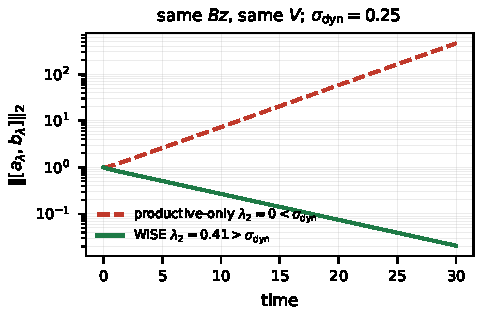
\includegraphics[width=0.78\columnwidth]{fig_modal.pdf}
  \caption{What that connectivity buys. Both assignments of Fig.~\ref{fig:flagship} share the
  served aggregate and productive value, differing only in $\lamtwo$. The critical mode
  of~\eqref{eq:modal} is propagated by exact matrix exponential from a common initial
  condition, gains fixed beforehand ($\sigmadyn=0.25$). The productively optimal assignment is
  not merely slow---it is \emph{unstable} ($\det A_{\lamtwo}<0$); WISE decays at the certified
  $\alpha=0.128$.}
  \label{fig:modal}
\end{figure}

\subsection{What connectivity buys: information-layer stability}
\begin{proposition}[Threshold and guaranteed rate]\label{thm:stability}
In the coordinates $a,b\in\R^{N-1}$ of $\mathbf1^{\perp}$, let a served-aggregate coordination
error $a$ be driven by a consensus estimator error $b$ diffusing over
$\widetilde L(z)=Q^{\top}\Lap(z)Q$:
\begin{equation}
\dot a=-\mF\,a+\vt_1 b,\qquad
\dot b=\vt_2\,a-c\,\widetilde L(z)\,b,
\label{eq:interconnection}
\end{equation}
with damping $\mF>0$, consensus gain $c>0$ and \emph{isotropic, mode-aligned} couplings
$\vt_1I,\vt_2I$, so \eqref{eq:interconnection} block-diagonalises in the eigenbasis of
$\widetilde L$: each eigenvalue $\lambda$ contributes an independent pair
\begin{equation}
\begin{bmatrix}\dot a_\lambda\\ \dot b_\lambda\end{bmatrix}
=A_\lambda\begin{bmatrix}a_\lambda\\ b_\lambda\end{bmatrix},\qquad
A_\lambda=\begin{bmatrix}-\mF&\vt_1\\ \vt_2&-c\lambda\end{bmatrix}.
\label{eq:modal}
\end{equation}
Since $\operatorname{tr}A_\lambda=-(\mF+c\lambda)<0$ and
$\det A_\lambda=c\,\mF\lambda-\vt_1\vt_2$, $A_\lambda$ is Hurwitz \emph{iff}
$\lambda>\sigmadyn:=\vt_1\vt_2/(c\,\mF)$, and its decay rate is
\begin{equation}
\alpha(\lambda)=\tfrac12\Big(\mF+c\lambda-
\sqrt{(\mF-c\lambda)^2+4\vt_1\vt_2}\Big).
\label{eq:rate}
\end{equation}
$\alpha$ is strictly increasing ($\alpha'=\tfrac c2[1-(c\lambda-\mF)/
\sqrt{(\mF-c\lambda)^2+4\vt_1\vt_2}]>0$) with $\alpha(\sigmadyn)=0$, so the whole
interconnection is exponentially stable iff $\lamtwo>\sigmadyn$, at rate $\ge\alpha(\lamtwo)$.
\end{proposition}
The two links must be kept apart. The relaxed selector gives a \emph{design and existence}
certificate ($\LamE\ge\sigmastar$: the fiber contains a fractional composition meeting the
requirement). The \emph{physical} guarantee attaches only to a realizable team: for integer
$\hat z$ passing direct re-certification with $\lamtwo(\Lap(\hat z))\ge\sigmastar>\sigmadyn$,
Lemma~\ref{lem:bridge} yields $\lamtwo(\Lgeo(q,\hat z))\ge\sigmastar$ at \emph{every}
admissible pose, hence the uniform rate $\alpha(\sigmastar)>0$. Lemma~\ref{lem:bridge} is
stated for integer $\hat z$ and is \emph{not} invoked at the fractional
$z^{\star}_{\mathrm{WISE}}$. This is the reduced information layer---not robot, load or
actuator dynamics.

\subsection{The price of self-sustainability}
\label{sec:price}
The lexicographic selector is exact, whereas a scalarised $V+\varepsilon\lamtwo$ recovers it
only as $\varepsilon\to0$ (Tikhonov~\cite{facchinei2003fvi}:
$\|Bz_\varepsilon-y^{\star}\|\le\sqrt{2\varepsilon\,\mathrm{osc}_{X_{\mathrm f}}(\lamtwo)/
\alpha}$, $\mathrm{osc}_{X_{\mathrm f}}(\lamtwo)=\LamX-\min_{X_{\mathrm f}}\lamtwo$), so a
finite $\varepsilon$ moves the aggregate (E6). Beyond the free fiber the requirement carries a
cost: with $\Price(\sigma)=V^{\star}-\max\{V(z):z\in X_{\mathrm f},\lamtwo(\Lap(z))\ge\sigma\}$
($+\infty$ if infeasible) and the capacities $\LamE\le\LamX=\max_{X_{\mathrm f}}\lamtwo$,

\begin{corollary}[Free/costly/impossible trichotomy]\label{thm:price}
$\Price$ is nondecreasing, proper and convex, with $\Price=0$ for $\sigma\le\LamE$ (free),
finite and positive for $\LamE<\sigma\le\LamX$ (costly), and $+\infty$ for $\sigma>\LamX$
(impossible). Under Slater the optimal multiplier satisfies
$\pi^{\star}\in\partial\Price(\sigma)$: the local sensitivity of optimal productive loss to the
connectivity requirement, in units of $V$.
\end{corollary}
\begin{proof}[Proof sketch]
The super-level set is convex and shrinks in $\sigma$, so $\Price$ is nondecreasing; $\sigma$
enters linearly, making $\Price$ a convex perturbation value whose subdifferential is the
optimal multiplier set. The cases are $\sigma\le\LamE$, $\sigma>\LamX$,
and between.
\end{proof}

\subsection{Finite-team recovery}
Rounding \emph{searches} for an integer $\hat z$ and re-checks it \emph{directly} against
budgets, occupancy, the lifted wrench LP~\eqref{eq:tensor} and $\lamtwo\ge\sigmastar$; if it
also satisfies $B\hat z=y^{\star}$ it is a zero-cost integer WISE, otherwise it carries a
\emph{recovery loss} $\ell(\hat z)=V^{\star}-V(\hat z)$, a quantity distinct from the integer
self-sustaining gap $g_{\mathbb Z}^{\mathrm{ss}}$. A Weyl/row-slack radius
$\|\hat z-z^{\star}\|_2<\min\{m_w/\kappa_w,\ m_\lambda/\kappa_L\}$ also certifies joint
feasibility a priori, but it is a worst-case bound---on our instances it certifies $0/30$ of
the recoveries that direct re-certification accepts---so we relegate it to the supplementary
material and treat direct re-certification as the operative finite-team test.

\subsection{Computing the certificate and recovering an integer team}
\label{sec:algorithm}

Stage~1 computes $z^{\mathrm{prod}}\in\arg\max_{X_{\mathrm f}}V$ and fixes
$y^{\star}=Bz^{\mathrm{prod}}$; the Stage-2 SDP~\eqref{eq:sdp} returns $\LamE$ and the
selector $z^{\star}_{\mathrm{WISE}}$, with $\LamE\ge\sigmastar$ the relaxed existence test.

\emph{Structured recovery.} One draw of \emph{occupancy-aware sequential randomized rounding}
processes robots in uniformly random order: robot $i$ samples from $z^{\star}_i$ restricted to
the currently available unit-capacity actions, idle always admissible, renormalizing after each
capacity update---so every draw meets one action per robot and all capacities exactly. A greedy
\emph{repair} then searches single-robot moves
$\mathcal D(\hat z)=\{e_{ir}{-}e_{ia}:\hat z_{ia}{=}1,\ r\ \text{a free relay}\}$, admitting
$d$ only if $\hat z{+}d\in\mathcal X$ with the lifted wrench LP~\eqref{eq:tensor} still
feasible, applying the admissible move that maximizes $\lamtwo$ and accepting it only if
$\Delta\lamtwo>\tau_\lambda$; as integer assignments are finite and $\lamtwo$ strictly
increases, the search cannot cycle ($K_{\max}{=}12$). The result is \emph{directly}
re-certified against budgets, wrench feasibility and $\lamtwo\ge\sigmastar$;
Proposition~\ref{prop:integer} is a separate, far more conservative radius. Repair trades
productive value for connectivity ($Bd\neq0$), so a recovered team is integer self-sustaining
but seldom \emph{exactly} zero-cost.

A fully \emph{distributed} realization---each robot sampling from a local flow over the graph
it forms---needs a convergence guarantee on a decision-dependent graph and is left to future
work; we claim only the centralized certificate.

\section{Simulation Study}
\label{sec:exp}

We validate on heterogeneous teams in a two-region world bridged only when a long-range type
relays; the heterogeneity is \emph{conflicting}---that type has both higher capacity and relay
gain---so WISE must reorganize a whole composition to free it. The headline metric is the
\emph{certified service rate}: the fraction of seeds re-certified both wrench-feasible
\emph{and} $m_\lambda:=\lamtwo(\Lap(z))-\sigmastar\ge0$. Over $30$ paired seeds
($N=12$) it is $100\%$ (Wilson $[89,100]$) for WISE-SDP at $V=V^{\star}$, against $0\%$
($[0,11]$) for the wrench-only, connectivity-only and \emph{scalar-capacity} selectors (the
last a greedy heuristic meeting $\|\wdem\|$ by scalar force totals, \emph{not} the
$V+\varepsilon\lamtwo$ scalarization of E4). Seeds are fixed and every reported number is
written to a manifest by the script producing
it.\footnote{Code, manifests and every generated number:
\url{https://github.com/jlmayorgaco/paper-P06-WISE-endogenous-wrench-equilibria}, tag
\texttt{v1.0-wise} (code and data commit \texttt{14fa38a3}); \texttt{make reproduce}
rebuilds them all and \texttt{make robot} reruns E2 from one command.}

\begin{figure*}[t]\centering
  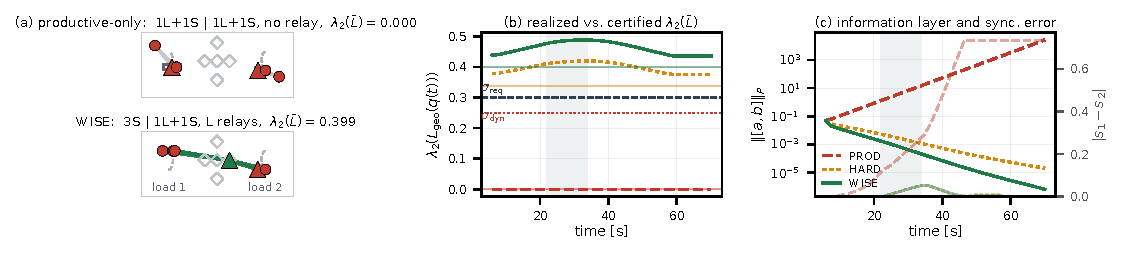
\includegraphics[width=\textwidth]{fig_robot_hero.pdf}
  \caption{Same productive optimum, three selectors. \textbf{(a)} The PROD--WISE exchange at
  the final pose: the scarce $L$ is the highest-productive-capacity type \emph{and} the only
  bridge, so both $L$ lifting disconnects the regions, whereas replacing one $L$ by two more $S$
  and sending the released $L$ to a relay preserves $Bz=y^{\star}$, $V^{\star}$ and both nominal
  wrench certificates. \textbf{(b)} $\lamtwo(\Lgeo(q(t)))$ against its certified surrogate
  $\lamtwo(\Lap)$ (thin, same colour). \textbf{(c)} $\|[a,b]\|_P$ (left, log; PROD exits at
  $5.3\cdot10^{5}$) and $|s_1{-}s_2|$ (right, faint); shading marks the disturbance.}
  \label{fig:hero}
\end{figure*}

\paragraph*{E1 --- Mechanism and networkability (Fig.~\ref{fig:hero}(a))}
The $N=6$ flagship comprises two loads---one torque-critical---and two long- plus four
short-range robots ($c_L=2c_S$), with $|\mathcal A|=12$. It admits an \emph{integer}, directly
re-certified, zero-cost assignment: replacing one long lifter by two additional short ones and
sending the released long robot to a relay site holds $Bz=(3,3)=y^{\star}$ and $V=V^{\star}$
exactly, both nominal wrench certificates granted by the inner-zonotope LP~\eqref{eq:tensor},
while $\lamtwo(\Lap)$ rises $0\to0.399$ (Thm.~\ref{thm:networkability},
$\Gamma_{\Emanifold}>0$). No rounding is needed: exhaustive enumeration of all
$|\mathcal A|^N=12^6=2.99\cdot10^6$ maps leaves $3864$ wrench-feasible, $1032$ on $\Emanifold$,
and $0.399$ is the \emph{integer} fiber capacity $\LamE^{\mathbb Z}=\max\{\lamtwo(\Lap(z)):
z\in\Emanifold\cap\{0,1\}^n\}$: a verified integer optimum, not a recovery. Enumeration
certifies $\LamE^{\mathbb Z}\le\LamE$, not the relaxed capacity---here tube infima depend on
\emph{both} endpoints' actions, so $\Lap$ is bilinear, not affine, and \eqref{eq:sdp} applies
only to the $N{=}12$ instances. On $200$ symmetric
$\lamtwo{=}\lambda_3$ instances the eigenspace criterion tracks the finite difference to median
error $10^{-6}$ against $0.04$ for a single eigenvector; on $12$ $N{=}12$ seeds \eqref{eq:iff}
holds $12/12$ ($\Gamma_{\Emanifold}\le3.4\cdot10^{-6}$ at the selector, $[0.45,1.78]$ at an
interior fiber point), with $\dim\Emanifold=59$ but $d_{\mathrm{net}}\in[10,12]$.

\paragraph*{E2 --- Planar closed-loop transport (Fig.~\ref{fig:hero}(b),(c))}
Two rigid loads with $M_k\dot\nu_k+D_k\nu_k=\sum_{i\in\mathcal C_k}A_{kh(i)}f_i+d_k(t)$ follow
separate curved paths. At each $20$\,Hz step a trajectory-PD wrench demand is realized by a
minimum-effort allocator restricted to the \emph{same} inner zonotope
$f_i\in U_{\tau(i)}^{\mathrm{in}}$ the certificate uses; $\Lgeo(q(t))$ is rebuilt from the
simulated poses and drives \eqref{eq:interconnection}, whose state shifts the normalized
path-progress command of each load's coalition (an illustrative downstream realization).
PROD, the hard-threshold HARD (cheapest relay site clearing $\sigmastar$,
declared tie-break) and WISE share all of that plus the disturbance and initial state, so only
the assignment differs; with $\sigmadyn=0.25$, $\sigmastar=0.30$ their surrogates are
$\lamtwo(\Lap)=0$, $0.336$, $0.399$ at identical $Bz$, $V$ and nominal certificates. Feasibility
is re-checked at \emph{every} control step: outside the declared disturbance window the demand
is met to $6\cdot10^{-8}$ (zero infeasible steps), inside it the team saturates (slack $0$,
peak residual $0.82$\,N) and the governor slows the load. \emph{(i)} Geometric transfer holds:
$\lamtwo(\Lgeo(q(t)))-\lamtwo(\Lap(\hat z))\ge+0.037$ at every operational step, no robot
leaving its tube. \emph{(ii)} The certified layer decays at fitted rates $0.156$ (WISE) and
$0.108$ (HARD), both above $\alpha(\sigmastar)=0.040$ (Cor.~\ref{cor:tv}), whereas PROD
\emph{grows} by $5.3\cdot10^{5}$. \emph{(iii)} WISE and HARD resynchronize to $|s_1{-}s_2|=0$
with both loads completing, while PROD's error grows to $0.734$ and load~1 never completes; a
random fiber point behaves like PROD ($\lamtwo=0$, error $0.641$): the degeneracy is not the
resource---the \emph{selection on it} is. Over $30$ paired worlds (mass $\pm10\%$, damping
$\pm15\%$, initial pose in the tubes, disturbance amplitude and onset; the seed/world is the
unit) every selector clearing the requirement---WISE, HARD, the tested $V+\varepsilon\lamtwo$
scalarization---succeeds $30/30$, against $0/30$ for PROD and the random point. Paired medians
over worlds (bootstrap, $20{,}000$ resamples) put WISE's peak
synchronization error $-0.733$ $[-0.749,-0.713]$ below PROD but $+1.7\cdot10^{-4}$
$[-2.5,5.5]\cdot10^{-4}$ against HARD---\emph{indistinguishable}---while its information-layer
rate is strictly higher, $+0.0478$ $[+0.0476,+0.0479]$. Past the threshold the extra margin
shows up there, not in the loads---but it is what degrades gracefully: under the predeclared
attenuation $L_{ir}(\rho)=(1{-}\rho)L_{ir}$, $\rho\in[0,0.6]$, everything else fixed, HARD
loses the certificate at $\rho=0.11$ and WISE at $\rho=0.27$. This simulates the modelled
layers, not a nonlinear robot--load theorem.

\paragraph*{E3 --- Integer recovery and an exact oracle}
At $N=12$, structured recovery over $30$ instances $\times\,30$ draws is jointly feasible in
$653/900$ before repair and $895/900$ after. Draws are nested within instances, so the
\emph{instance} is the unit: the mean per-instance rate is $99.4\%$ (cluster bootstrap
$[98.3,100.0]$), all $30$ succeeding on $\ge1$ draw. Recovery loss is median $4.2\%$ and only
$83/895$ recoveries are exactly zero-cost---a property of the heuristic, not of the attainable
integer optimum---while the worst-case radius certifies $0/30$ seeds. For $N\le8$ an exact
oracle enumerates \emph{every} $|\mathcal A|^N$ map: no false positives at the design
requirement ($0/23$) and $\max g_{\mathbb Z}^{\mathrm{ss}}<0.06\%$ of $V^{\star}$; pushed
\emph{adversarially} to $\sigma=0.97\LamE$ it is integer-tight at $N{=}6$ in only $13/50$
cases, never at $N{=}7,8$.

\paragraph*{E4 --- Regimes, price and scalarization}
Sweeping the long-range-type fraction $\nu\in[0.17,0.67]$ against the wrench-demand multiplier
$\tau_d\in[1,4]$ ($6\times6$ cells, $4$ seeds) activates no wrench facet, so at \emph{fixed}
$(\nu,\text{seed})$ the value $\LamE$ is invariant along $\tau_d$ (spread $\le2\cdot10^{-8}$;
grid mean $1.572$) while across $\nu$ its per-$\nu$ mean rises $0.82\to2.48$ and the costly
band widens $0.10\to0.97$: scarcity compresses \emph{both} the free and the merely-expensive
regime. At $\tau_d=8$ the first wrench facet binds, preserving the local fiber dimension but
shortening its global reach ($\LamE$ falls $10$--$20\%$). Over $40$ further seeds $\Price$
traces the predicted shape, its dual matching the finite difference over $84$ points
($r=0.996$). Two controls close the loop: the hard connectivity-constrained optimum also
reaches $V^{\star}$ but returns \emph{any} point of that face ($m_\lambda=+0.15$ versus WISE's
$+2.55$), and a scalarized $V+\varepsilon\lamtwo$ \emph{can} perturb the aggregate---every
tested $\varepsilon\in[10^{-3},1]$ gave nonzero drift ($2\cdot10^{-4}$ to $0.284$), consistent
with the local quadratic geometry of $V$: aggregate displacement is first-order in the
perturbation, productive loss second-order near the interior optimum. That drift is a property
of the relaxation---over E2's \emph{integer} action set the same selector returns the WISE
point at every $\varepsilon$---and WISE needs no weight to calibrate.

\section{Conclusion}
\label{sec:conclusion}

We identified composition degeneracy as a resource in heterogeneous cooperative transport:
when the productive optimum fixes the served aggregate but not its composition
(Theorem~\ref{thm:degeneracy}), a spectral program selects, among equally productive
assignments, one that preserves the estimator's communication substrate; relaxed WISE
existence and selection reduce to a semidefinite program (Theorem~\ref{thm:existence}), and
a small-gain condition ties the requirement to optimizer--estimator stability
(Proposition~\ref{thm:stability}).

\paragraph*{Limitations and future work}
The guarantees hold for the relaxed candidate-site model ($\Lap(z)$ is within a bounded
perturbation $\varepsilon_L$ of $\Lgeo(q)$ under Lemma~\ref{lem:bridge}, with
$\varepsilon_L$ measured, not bounded a priori; integers are re-certified after rounding,
Remark~\ref{rem:integer}); nonholonomic realizability is modelled, not proved; validation
is in simulation. An a-priori mismatch bound, a nonholonomic realizability theorem, and
hardware validation remain open.

\bibliographystyle{IEEEtran}
\bibliography{references}

\end{document}
